% begin module approximate integration
\begin{frame}
\frametitle{Approximate Integration}

Here, we present some methods
for finding approximate values of definite integrals.  Such methods are
needed when an antiderivative for the integrand is hard or impossible 
to compute:
\[
\int_a^b e^{t^2}\; dt \;\;\;\;\int_a^b \sin(x^2)\;dx
\]
(This does not mean that, for example, there is 
no function whose derivative is $e^{x^2}$;  there certainly is.
 We just can't write it down nicely--in terms of `elementary functions'. 
)\\
Another need may arise when the integrand is not known by a formula but only by a
table of values obtained, say, from a scientific experiment.\\

What we need is an efficient method to estimate area when we 
can not find the antiderivative.

\end{frame}

% % % % % % % % % % % % % % % % % % % % % % % % % % % % % % % %
\begin{frame}
\frametitle{Left and Right approximations}
Let $f$ be a continuous function on $[a,b]$.  Recall that the definite integral is defined as
\[
\int_a^b f(x)dx = \lim_{n\to \infty} \sum\limits_{i=1}^n
f(x_i^*)\Delta x
\]   
where $[a,b]$ has been divided into $n$ subintervals
$[x_{i-1},x_i]$ of equal length $\Delta x=(b-a)/n$, and $x_i^*$ is any
point in $[x_{i-1},x_i]$.\\ \pause 

Recall: If each $ x_i^* $ is chosen to be the right endpoint of the interval, $ x_i^* = x_{i}$   then we get the Right endpoint approximation 
\[
\int_a^b  f(x)\; dx \approx R_N  = \sum\limits_{i=1}^n f(x_{i})\Delta x
\]

\pause 
If each $ x_i^* $ is chosen to be the left endpoint of the interval, $ x_i^* = x_{i-1}$   then we get the Left endpoint approximation 
\[
\int_a^b f(x)\; dx \approx L_N = \sum\limits_{i=1}^n f(x_{i-1})\Delta x
\]

\end{frame}
% % % % % % % % % % % % % % % % % % % % % % % % % % % % % % % %
% % % % % % % % % % % % % % % % % % % % % % % % % % % % % % % %
\begin{frame}
\frametitle{Left and Right endpoint approximations}

\begin{tikzpicture}[scale=.8]
\coordinate (p1) at (0.7,3);
\coordinate (p2) at (1,3.3);
\coordinate (p3) at (2,2.5);
\coordinate (p4) at (3,2.5);
\coordinate (p5) at (4,3.5);
\coordinate (p6) at (5,4.1);
\coordinate (p7) at (6,3.4);
\coordinate (p8) at (7,4.1);
\coordinate (p9) at (8,4.6);
\coordinate (p10) at (9,4);
\coordinate (p11) at (9.5,4.7);

% The cyan background
%\fill[cyan!10] 
%  (p2|-0,0) -- (p2) -- (p3) -- (p4) -- (p5) -- (p6) -- (p7) -- (p8) -- (p9) -- (p10) -- (p10|-0,0) -- cycle;
% the broken line connecting points on the curve
  \draw[fill=cyan!10] (1,0) -- (p2) -- ($(p2)+(1,0)$) -- (p3)-- ($(p3)+(1,0)$) -- (p4)-- ($(p4)+(1,0)$) -- (p5) -- ($(p5)+(1,0)$) -- (p6) -- ($(p6)+(1,0)$) -- (p7) -- ($(p7)+(1,0)$) -- (p8)-- ($(p8)+(1,0)$) -- (p9)-- ($(p9)+(1,0)$) -- (p10)--(9,0) -- cycle;
% the dark cyan stripe
\fill[cyan!30] (p6|-0,0) -- (p6) -- ($(p6)+(1,0)$) -- (p7|-0,0) -- cycle;  
% vertical lines and labels
\foreach \n/\texto in {2/{a=x_0},3/{x_1},4/{},5/{},6/{x_{j-1}},7/{x_j},8/{},9/{x_{n-1}},10/{b=x_n}}
{
  \draw (p\n|-0,0) -- (p\n);
  \node[below,text height=1.5ex,text depth=1ex,font=\small] at (p\n|-0,0) {$\texto$};
}
% the curve
\draw[thick,cyan] 
  %(p1) to[out=70,in=180] 
  (p2) to[out=0,in=150] 
  (p3) to[out=-50,in=230] (p4) to[out=30,in=220] 
  (p5) to[out=50,in=150] (p6) to[out=-30,in=180] 
  (p7) to[out=0,in=230] (p8) to[out=40,in=180] 
  (p9) to[out=-30,in=180] (p10); 
  % to[out=0,in=260] (p11);
% The axes
\draw[->] (-0.5,0) -- (10,0) coordinate (x axis);
\draw[->] (0,-0.5) -- (0,6) coordinate (y axis);
% labels for the axes
\node[below] at (x axis) {$x$};
\node[left] at (y axis) {$y$};
% label for the function
\node[above,text=cyan] at (p11) {$y=f(x)$};
\end{tikzpicture}
\[
\int_a^b f(x)\; dx \approx L_N = \sum\limits_{i=1}^n f(x_{i-1})\Delta x
\]
\end{frame}

\begin{frame}
\begin{tikzpicture}[scale=.8]
\coordinate (p1) at (0.7,3);
\coordinate (p2) at (1,3.3);
\coordinate (p3) at (2,2.5);
\coordinate (p4) at (3,2.5);
\coordinate (p5) at (4,3.5);
\coordinate (p6) at (5,4.1);
\coordinate (p7) at (6,3.4);
\coordinate (p8) at (7,4.1);
\coordinate (p9) at (8,4.6);
\coordinate (p10) at (9,4);
\coordinate (p11) at (9.5,4.7);

% The cyan background
%\fill[cyan!10] 
%  (p2|-0,0) -- (p2) -- (p3) -- (p4) -- (p5) -- (p6) -- (p7) -- (p8) -- (p9) -- (p10) -- (p10|-0,0) -- cycle;

% the broken line connecting points on the curve
  \draw[fill=cyan!10] (1,0) -- ($(p3)+(-1,0)$)-- (p3) -- ($(p4)+(-1,0)$) -- (p4)-- ($(p5)+(-1,0)$) -- (p5)-- ($(p6)+(-1,0)$) -- (p6) -- ($(p7)+(-1,0)$) -- (p7) -- ($(p8)+(-1,0)$) -- (p8)-- ($(p9)+(-1,0)$) -- (p9)-- ($(p10)+(-1,0)$) -- (p10)--(9,0) -- cycle;
% the dark cyan stripe
  \fill[cyan!30] (p6|-0,0) -- ($(p7)+(-1,0)$) -- (p7) -- (p7|-0,0) -- cycle;  
% vertical lines and labels
\foreach \n/\texto in {2/{a=x_0},3/{x_1},4/{},5/{},6/{x_{j-1}},7/{x_j},8/{},9/{x_{n-1}},10/{b=x_n}}
{
  \draw (p\n|-0,0) -- (p\n);
  \node[below,text height=1.5ex,text depth=1ex,font=\small] at (p\n|-0,0) {$\texto$};
}
% the curve
\draw[thick,cyan] 
    %(p1) to[out=70,in=180] 
    (p2) to[out=0,in=150] 
    (p3) to[out=-50,in=230] (p4) to[out=30,in=220] 
    (p5) to[out=50,in=150] (p6) to[out=-30,in=180] 
    (p7) to[out=0,in=230] (p8) to[out=40,in=180] 
    (p9) to[out=-30,in=180] (p10); 
    % to[out=0,in=260] (p11);
% The axes
\draw[->] (-0.5,0) -- (10,0) coordinate (x axis);
\draw[->] (0,-0.5) -- (0,6) coordinate (y axis);
% labels for the axes
\node[below] at (x axis) {$x$};
\node[left] at (y axis) {$y$};
% label for the function
\node[above,text=cyan] at (p11) {$y=f(x)$};
\end{tikzpicture}
\[
\int_a^b  f(x)\; dx \approx R_N  = \sum\limits_{i=1}^n f(x_{i})\Delta x
\]
\end{frame}

\begin{frame}

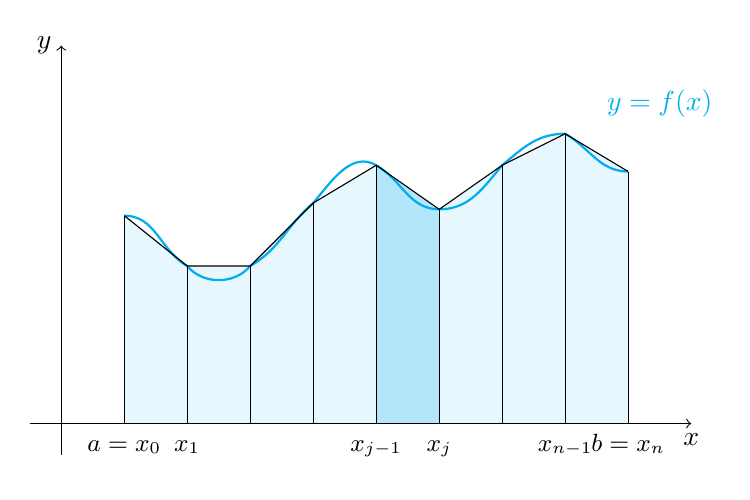
\begin{tikzpicture}[scale=.8]
\coordinate (p1) at (0.7,3);
\coordinate (p2) at (1,3.3);
\coordinate (p3) at (2,2.5);
\coordinate (p4) at (3,2.5);
\coordinate (p5) at (4,3.5);
\coordinate (p6) at (5,4.1);
\coordinate (p7) at (6,3.4);
\coordinate (p8) at (7,4.1);
\coordinate (p9) at (8,4.6);
\coordinate (p10) at (9,4);
\coordinate (p11) at (9.5,4.7);

% The cyan background
\fill[cyan!10] 
  (p2|-0,0) -- (p2) -- (p3) -- (p4) -- (p5) -- (p6) -- (p7) -- (p8) -- (p9) -- (p10) -- (p10|-0,0) -- cycle;
% the dark cyan stripe
\fill[cyan!30] (p6|-0,0) -- (p6) -- (p7) -- (p7|-0,0) -- cycle;
% the curve
\draw[thick,cyan] 
    %(p1) to[out=70,in=180] 
    (p2) to[out=0,in=150] 
    (p3) to[out=-50,in=230] (p4) to[out=30,in=220] 
    (p5) to[out=50,in=150] (p6) to[out=-30,in=180] 
    (p7) to[out=0,in=230] (p8) to[out=40,in=180] 
    (p9) to[out=-30,in=180] (p10); 
    % to[out=0,in=260] (p11);
% the broken line connecting points on the curve
\draw (p2) -- (p3) -- (p4) -- (p5) -- (p6) -- (p7) -- (p8) -- (p9) -- (p10);
% vertical lines and labels
\foreach \n/\texto in {2/{a=x_0},3/{x_1},4/{},5/{},6/{x_{j-1}},7/{x_j},8/{},9/{x_{n-1}},10/{b=x_n}}
{
  \draw (p\n|-0,0) -- (p\n);
  \node[below,text height=1.5ex,text depth=1ex,font=\small] at (p\n|-0,0) {$\texto$};
}
% The axes
\draw[->] (-0.5,0) -- (10,0) coordinate (x axis);
\draw[->] (0,-0.5) -- (0,6) coordinate (y axis);
% labels for the axes
\node[below] at (x axis) {$x$};
\node[left] at (y axis) {$y$};
% label for the function
\node[above,text=cyan] at (p11) {$y=f(x)$};
\end{tikzpicture}

\end{frame}
% % % % % % % % % % % % % % % % % % % % % % % % % % % % % % % %
\begin{frame}

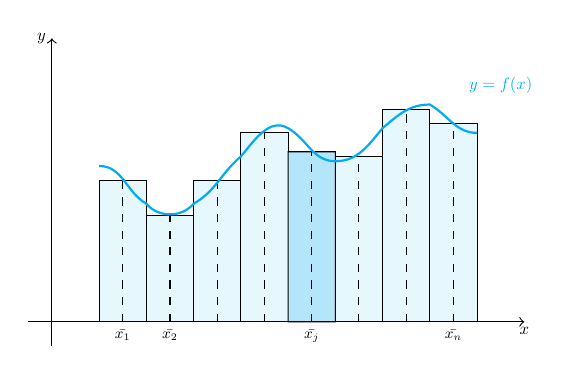
\begin{tikzpicture}[scale=.6, every node/.style={scale=0.6}]


\coordinate (p1) at (0.7,3);
\coordinate (p2) at (1,3.3);
\coordinate (p3) at (2,2.5);
\coordinate (p4) at (3,2.5);
\coordinate (p5) at (4,3.5);
\coordinate (p6) at (5,4.1);
\coordinate (p7) at (6,3.4);
\coordinate (p8) at (7,4.1);
\coordinate (p9) at (8,4.6);
\coordinate (p10) at (9,4);
\coordinate (p11) at (9.5,4.7);

% The cyan background
%\fill[cyan!10] 
%  (p2|-0,0) -- (p2) -- (p3) -- (p4) -- (p5) -- (p6) -- (p7) -- (p8) -- (p9) -- (p10) -- (p10|-0,0) -- cycle;


% the broken line connecting points on the curve
 \draw[fill=cyan!10] (1,0) --(1,3)--(2,3)--(2,0)--(2,2.25)--(3,2.25)--(3,0)--(3,3)--(4,3)--(4,0)--(4,4)--(5,4)--(5,0)--(5,3.6)--(6,3.6)--(6,0)--(6,3.5)--(7,3.5)--(7,0)--(7,4.5)--(8,4.5)--(8,0)--(8,4.2)--(9,4.2) --(9,0) -- cycle;
 % the dark cyan stripe
 \fill[cyan!30,draw=black] (p6|-0,0) -- (5,3.6) -- (6,3.6) -- (p7|-0,0) -- cycle;
% vertical lines and labels
\draw[dashed] (1.5,0) -- (1.5,3);
\node[below,text height=1.5ex,text depth=1ex,font=\small] at (1.5,0) {$\bar{x_1}$};
\draw[dashed] (2.5,0) -- (2.5,2.25);
\node[below,text height=1.5ex,text depth=1ex,font=\small] at (2.5,0) {$\bar{x_2}$};
\draw[dashed] (3.5,0) -- (3.5,3);
\node[below,text height=1.5ex,text depth=1ex,font=\small] at (3.5,0) { };
\draw[dashed] (4.5,0) -- (4.5,4);
\node[below,text height=1.5ex,text depth=1ex,font=\small] at (4.5,0) { };
\draw[dashed] (5.5,0) -- (5.5,3.6);
\node[below,text height=1.5ex,text depth=1ex,font=\small] at (5.5,0) {$\bar{x_j}$};
\draw[dashed] (6.5,0) -- (6.5,3.5);
\node[below,text height=1.5ex,text depth=1ex,font=\small] at (6.5,0) { };
\draw[dashed] (7.5,0) -- (7.5,4.5);
\node[below,text height=1.5ex,text depth=1ex,font=\small] at (7.5,0) { };
\draw[dashed] (8.5,0) -- (8.5,4.2);
\node[below,text height=1.5ex,text depth=1ex,font=\small] at (8.5,0) {$\bar{x_n}$};

% the curve
\draw[thick,cyan] 
   %(p1) to[out=70,in=180] 
   (p2) to[out=0,in=150] 
   (p3) to[out=-50,in=230] (p4) to[out=30,in=220] 
   (p5) to[out=50,in=150] (p6) to[out=-30,in=180] 
   (p7) to[out=0,in=230] (p8) to[out=40,in=180] 
   (p9) to[out=-30,in=180] (p10); 
   % to[out=0,in=260] (p11);
% The axes
\draw[->] (-0.5,0) -- (10,0) coordinate (x axis);
\draw[->] (0,-0.5) -- (0,6) coordinate (y axis);
% labels for the axes
\node[below] at (x axis) {$x$};
\node[left] at (y axis) {$y$};
% label for the function
\node[above,text=cyan] at (p11) {$y=f(x)$};

%\draw[help lines,step=.2] (-2,-2) grid (12,12);
\end{tikzpicture}

\end{frame}
% % % % % % % % % % % % % % % % % % % % % % % % % % % % % % % %

